\documentclass{beamer}
\usepackage{amsmath, amssymb, amsthm, mathtools}
\usepackage{subfigure}
\usepackage{graphicx}
\usepackage{caption}
\usepackage{cancel}
% \usepackage{subcaption}

\newcommand{\bs}[1]{\boldsymbol{#1}}
\newcommand{\norm}[1]{\left\| #1 \right\|}
\newcommand{\snorm}[1]{\left| #1 \right|}
\newcommand{\LRp}[1]{\left( #1 \right)}
\newcommand{\LRs}[1]{\left[ #1 \right]}
\newcommand{\LRc}[1]{\left\{ #1 \right\}}
\newcommand{\Grad}{\ensuremath{\nabla}}
\newcommand{\Div}{\ensuremath{\nabla\cdot}}
\newcommand{\bfn}{\mbox{\boldmath $n$}}
\newcommand{\bfH}{\mbox{\boldmath $H$}}
\newcommand{\HdivK}{\bfH(\text{div},K)}
\newcommand{\HOneK}{H^{-1}(K)}
\newcommand{\HOneOmegah}{H^{-1}(\Omega_h)}
\newcommand{\HdivOmegah}{\bfH(\text{div},\Omega_h)}
\newcommand{\vdeltau}{v_{\delta\bs u_h}}
\newcommand{\taudeltau}{\btau_{\delta\bs u_h}}
\newcommand{\ip}[1]{\left\langle #1 \right\rangle}
\newcommand{\pd}[2]{\frac{\partial#1}{\partial#2}}
\newcommand{\pdd}[3]{\frac{\partial^2#1}{\partial#2\partial#3}}

\def\arr#1#2#3#4{\left[
\begin{array}{cc}
#1 & #2\\
#3 & #4\\
\end{array}
\right]}
\def\vecttwo#1#2{\left[
\begin{array}{c}
#1\\
#2\\
\end{array}
\right]}
\def\vectthree#1#2#3{\left[
\begin{array}{c}
#1\\
#2\\
#3\\
\end{array}
\right]}

\renewcommand{\arraystretch}{2.0}

\def\etal{{\it et al.~}}

\usetheme[secheader]{pecostalk}

\def\nut{\tilde\nu}

\author[Truman E. Ellis]{Truman E. Ellis}
\title[Intro to Turbulence Modeling]{Introduction to Turbulence Modeling}
\subtitle{or Why Turbulence Modeling is Black Magic}
\institute{Institute for Computational and Engineering Sciences\\
The University of Texas at Austin}

\begin{document}

\begin{frame}
\titlepage
\end{frame}

\begin{frame}
\frametitle{Reynolds Averaged Navier Stokes}
Let $\phi=\bar \phi+\phi'$, where
\begin{equation*}
\bar \phi=\lim_{T\rightarrow\infty}\int_{t_0}^{t_0+T}\phi(t)\,dt
\end{equation*}
Interested in solving for $\bar u_i$. Nondimensionalizing such that $\rho=1$,
\begin{columns}[T]
\begin{column}{0.29\textwidth}
\begin{block}{Continuity Equation}
\begin{equation*}
\pd{u_i}{x_i}=0
\end{equation*}
\vspace{0.05ex}
\[
\Downarrow
\]
\vspace{0.05ex}
\begin{equation*}
\pd{\bar u_i}{x_i}=0
\end{equation*}
\end{block}
\end{column}
\begin{column}{0.64\textwidth}
\begin{block}{Momentum Equation}
\begin{equation*}
\pd{u_i}{t}+u_j\pd{u_i}{x_j}=-\pd{p}{x_i}+\frac{1}{Re}\frac{\partial^2 u_i}{\partial x_j\partial x_i}
\end{equation*}
\vspace{-0.5ex}
\[
\Downarrow
\]
\vspace{-0.5ex}
\begin{equation*}
\pd{\bar u}{t}+\bar u_j\pd{\bar u_i}{x_j}=-\pd{\bar p}{x_i}
+\pd{}{x_j}\left[-\overline{u_i'u_j'}+\frac{1}{Re}\pd{\bar u_i}{x_j}\right]
\end{equation*}
\end{block}
\end{column}
\end{columns}
\vspace{1ex}
But the Reynolds stress, $\overline{u_i'u_j'}$ is an unclosed quantity.
\end{frame}

\begin{frame}\frametitle{Modeling the Reynolds Stress}
\begin{equation*}
\pd{\bar u}{t}+\bar u_j\pd{\bar u_i}{x_j}=-\pd{\bar p}{x_i}
+\pd{}{x_j}\left[-\overline{u_i'u_j'}
+\frac{1}{Re}\left(\pd{\bar u_i}{x_j}+\pd{\bar u_j}{x_i}\right)\right]
\end{equation*}
\begin{block}{Eddy Viscosity Hypothesis}
\begin{equation*}
\overline{u_i'u_j'}=-\nu_T\left(\pd{\bar u_i}{x_j}+\pd{\bar u_j}{x_i}\right)
+\frac{2k}{3}\delta_{ij}
\end{equation*}
where $k=\frac{1}{2}\overline{u_i'u_i'}$.
\end{block}
This assumption is fundamentally flawed, but useful.

\vspace{2ex}
We still need a model for $\nu_T$ and $k$.
\end{frame}

\begin{frame}\frametitle{Spalart-Allmaras Model}
\begin{itemize}
	\item Model the eddy viscosity
	\item Assume $k$ is negligible
	\item Surprisingly decent for the types of flows it was designed for (external aerodynamics)
\end{itemize}
\begin{align*}
\pd{\nut}{t}+\bar u_j\pd{\nut}{x_j}&=C_{b1}[1-f_{t2}]\tilde S\nut+\frac{1}{\sigma}
\left\{\Div[(\nu+\nut)\Grad\nut]+C_{b2}\snorm{\Grad\nut}^2\right\}\\
&-\left[C_{w1}f_{w}-\frac{C_{b1}}{\kappa^2}f_{t2}\right]\left(\frac{\nut}{d}\right)^2+f_{t1}\Delta U^2
\end{align*}
\begin{equation*}
\nu_T=\nut f_{v1},\quad f_{v1}=\frac{\chi^3}{\chi^3+v_{v1}^3},
\quad \chi=\frac{\nut}{\nu}\quad\cdots
\end{equation*}
\end{frame}

\begin{frame}[shrink=5]\frametitle{$k-\epsilon$ Exact Equations}
\begin{block}{Turbulence Kinetic Energy Equation}
\begin{equation*}
\pd{k}{t}+\bar u_i\pd{k}{x_i}=-\overline{u_i'u_j'}\pd{\bar u_i}{x_j}
-\pd{}{x_i}\left(\frac{1}{2}\overline{u_j'u_j'u_i'}+\overline{p'u_i'}\right)
+\nu\frac{\partial^2 k}{\partial x_i\partial x_i}-\epsilon
\end{equation*}
\end{block}
\begin{block}{Dissipation Equation}
\begin{equation*}
\pd{\epsilon}{t}+\bar u_i\pd{\epsilon}{x_i}=\nu\frac{\partial^2\epsilon}{\partial x_i\partial x_i}
+P_{\epsilon}+D_{\epsilon}-\Phi_\epsilon
\end{equation*}
\[
P_\epsilon=-2\nu\LRs{\overline{\pd{u_i'}{x_j}\pd{u_k'}{x_j}}\pd{\bar u_i}{x_k}
+\overline{\pd{u_j'}{x_i}\pd{u_j'}{x_k}}\pd{\bar u_i}{x_k}
+\overline{u_k'\pd{u_i'}{x_j}}\pdd{\bar u_i}{x_k}{x_j}
+\overline{\pd{u_i'}{x_k}\pd{u_i'}{x_m}\pd{u_k'}{x_m}}
}
\]
\[
D_\epsilon=-\pd{}{x_k}\LRp{\overline{u_k'\epsilon'}+2\nu\overline{\pd{p'}{x_m}\pd{u_k'}{x_m}}}
\]
\[
\Phi_\epsilon=2\nu^2\overline{\pdd{u_i'}{x_k}{x_m}\pdd{u_i'}{x_k}{x_m}}
\]
\end{block}
\end{frame}

\begin{frame}[shrink=5]\frametitle{$k-\epsilon$ Approximations}
\begin{block}{Turbulence Kinetic Energy Equation}
\[
\frac{1}{2}\overline{u_j'u_j'u_i'}+\overline{p'u_i'}\approx-\frac{\nu_T}{\sigma_k}\pd{k}{x_i}
\]
\end{block}
\begin{block}{Dissipation Equation}
From dimensional analysis
\[
\nu_T\approx C_\mu\frac{k^2}{\epsilon}
\]
\[
P_\epsilon\approx-C_{\epsilon1}\frac{\epsilon}{k}\overline{u_i'u_j'}\pd{\bar u_i}{x_j}
\]
\[
\Phi_\epsilon\approx C_{\epsilon2}\frac{\epsilon^2}{k}
\]
From gradient transport model
\[
D_\epsilon\approx\pd{}{x_i}\LRp{\frac{\nu_T}{\sigma_\epsilon}\pd{\epsilon}{x_i}}
\]
\end{block}
\end{frame}

\begin{frame}\frametitle{Channel Flow Predictions}
\begin{columns}[c]
\begin{column}{0.7\textwidth}
\begin{figure}[t]
	\begin{center}
		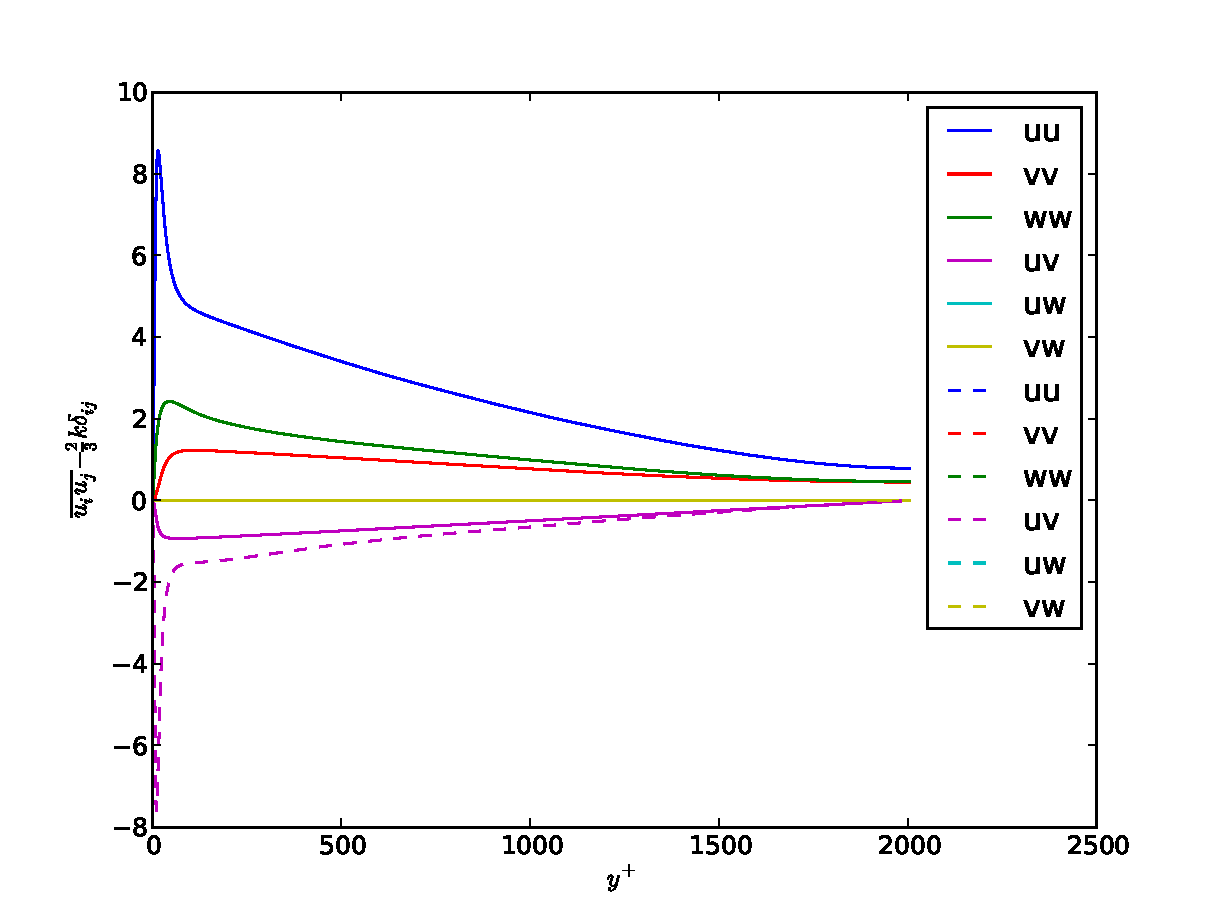
\includegraphics[width=\textwidth]{ReynoldsStress.pdf}
	\end{center}
	\caption{Reynolds Stress Components}
\end{figure}
\end{column}
\hspace{-3em}
\begin{column}{0.3\textwidth}
\begin{align*}
&\overline{u_i'u_j'}-\frac{2}{3}k\delta_{ij}\\
&\approx-\nu_T\LRp{\pd{\bar u_i}{x_j}+\pd{\bar u_j}{x_i}}
\end{align*}
\end{column}
\end{columns}
\end{frame}

\begin{frame}\frametitle{Channel Flow Predictions}
\begin{columns}[c]
\begin{column}{0.7\textwidth}
\begin{figure}[t]
	\begin{center}
		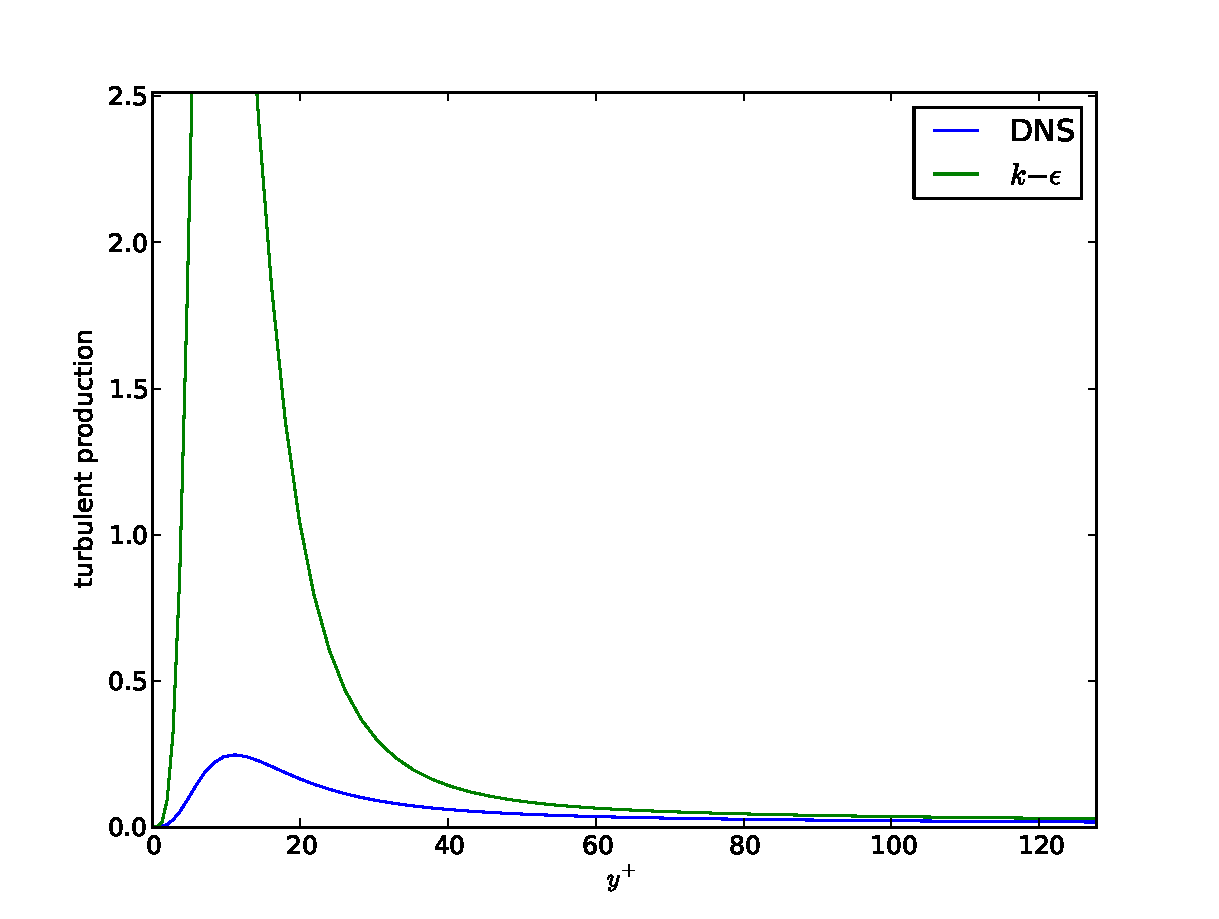
\includegraphics[width=\textwidth]{Production.pdf}
	\end{center}
	\caption{Production of Turbulent Kinetic Energy}
\end{figure}
\end{column}
\hspace{-3em}
\begin{column}{0.3\textwidth}
\begin{align*}
&\overline{u_i'u_j'}\pd{\bar u_i}{x_j}\approx\\
&C_\mu\frac{k^2}{\epsilon}\LRp{\pd{\bar u_i}{x_j}+\pd{\bar u_j}{x_i}}\pd{\bar u_i}{x_j}
\end{align*}
\end{column}
\end{columns}
\end{frame}

\begin{frame}\frametitle{Channel Flow Predictions}
\begin{columns}[c]
\begin{column}{0.7\textwidth}
\begin{figure}[t]
	\begin{center}
		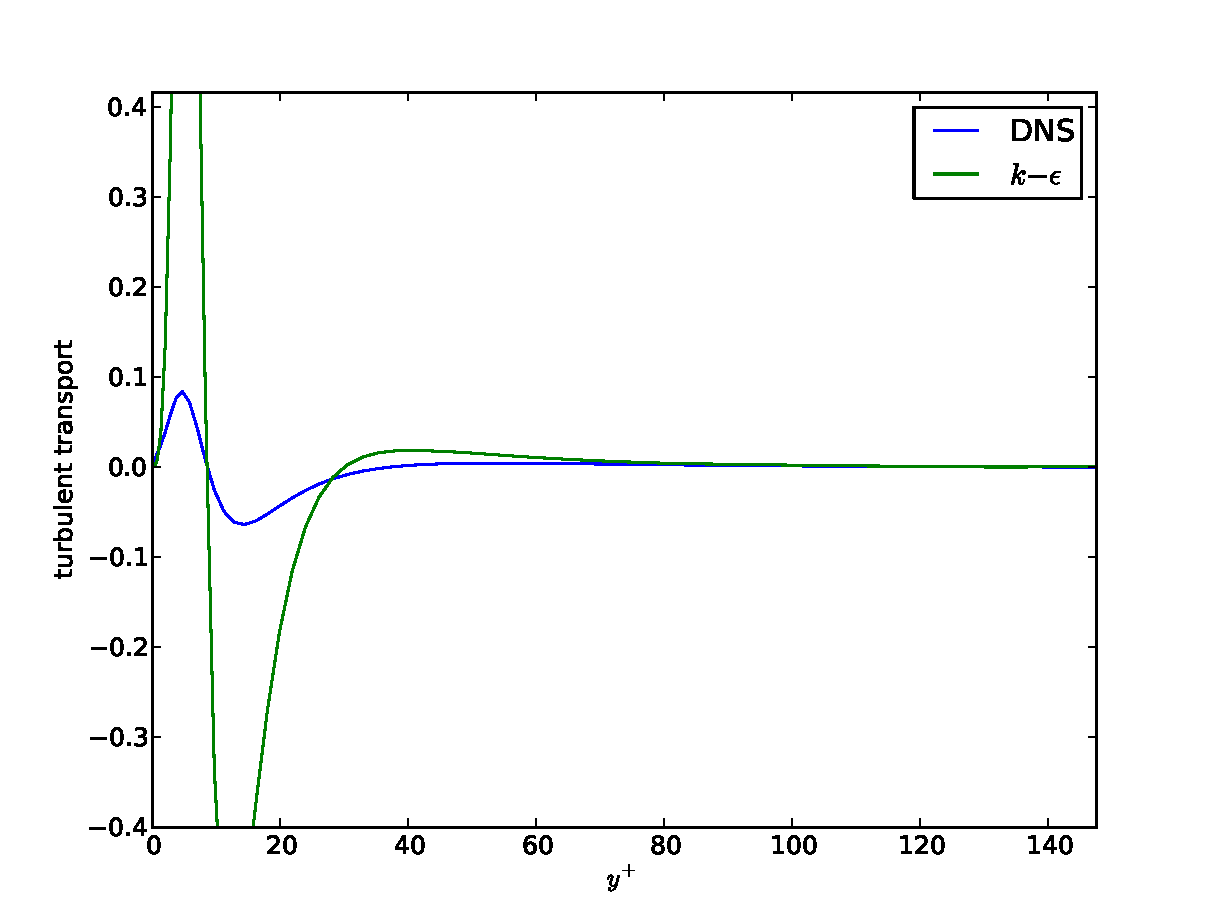
\includegraphics[width=\textwidth]{Transport.pdf}
	\end{center}
	\caption{Transport of Turbulent Kinetic Energy}
\end{figure}
\end{column}
\hspace{-3em}
\begin{column}{0.3\textwidth}
\begin{align*}
&\pd{}{x_i}\LRp{\frac{1}{2}\overline{u_k'u_k'u_i'}+\overline{p'u_i'}}\\
&\approx-\pd{}{x_i}\LRp{\frac{\nu_T}{\sigma_k}\pd{k}{x_i}}
\end{align*}
\end{column}
\end{columns}
\end{frame}

\begin{frame}\frametitle{Notes on $k-\epsilon$}
\begin{block}{Fixes near the wall}
\begin{itemize}
	\item Wall functions
	\item Two-layer models
	\item SST $k-\omega$
	\item $\overline{v^2}-f$ four equation model ($f$ is an elliptic relaxation function)
\end{itemize}
\end{block}
\begin{block}{Boundary conditions}
\begin{itemize}
	\item BC on $\epsilon$ is not obvious
	\item Enforce both $k=0$ and $\pd{k}{n}=0$ at walls.
\end{itemize}
\end{block}
\begin{block}{Popularity}
\begin{itemize}
	\item One of the earliest models
	\item Physically motivated derivation
	\item Insensitive to freestream conditions on $k$ and $\epsilon$
\end{itemize}
\end{block}
\end{frame}

\begin{frame}\frametitle{Wilcox (1993) $k-\omega$ Model }
\begin{block}{Turbulence Kinetic Energy Equation}
\[
\pd{k}{t}+\bar u_j\pd{k}{x_j}=2\nu_T\snorm{S}^2-C_\mu k\omega
+\pd{}{x_j}\LRp{\LRp{\nu+\frac{\nu_T}{\sigma_k}}\pd{k}{x_j}}
\]
\end{block}
\begin{block}{Specific Dissipation Equation}
\[
\pd{\omega}{t}+\bar u_j\pd{\omega}{x_j}=2C_{\omega1}\snorm{S}^2-C_{\omega2}\omega^2
+\pd{}{x_j}\LRp{\LRp{\nu+\frac{\nu_T}{\sigma_\omega}}\pd{\omega}{x_j}}
\]
\[
\omega\equiv\frac{\epsilon}{C_\mu k}
\]
\[
\nu_T=\frac{k}{\omega}
\]
\end{block}
\end{frame}

\begin{frame}\frametitle{Notes on $k-\omega$}
\begin{block}{Wall Treatment}
\begin{itemize}
	\item Produces decent results at the wall
	\item Formally, $\omega$ is singular at a perfectly smooth wall
	\item Numerically, this is fixed by assuming a finite roughness
	\begin{itemize}
		\item $\omega_{wall}=\frac{40000\nu_{wall}}{k_s^2}$, need $\frac{u_\tau k_s}{\nu}<5$
	\end{itemize}
	\item Can perform the same trick with two BCs on $k$
\end{itemize}
\end{block}

\begin{block}{Other Notes}
\begin{itemize}
	\item Early models were very sensitive to freestream conditions on $\omega$
	\item Menter propsed \emph{shear stress transport} model to overcome this shortcoming
	\item Possible to write a $k-\epsilon$ model with $k-\omega$ ``physics''
\end{itemize}
\end{block}
\end{frame}

\begin{frame}\frametitle{Other Ideas -- Unsteady RANS}
\begin{figure}[t]
	\begin{center}
		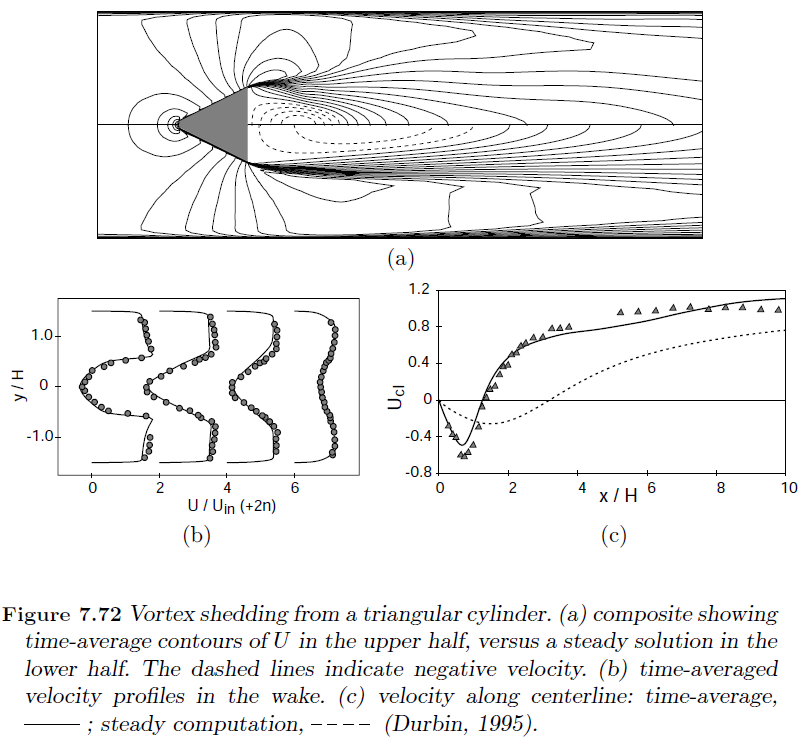
\includegraphics[height=0.9\textheight]{URANS.png}
	\end{center}
\end{figure}
\end{frame}

\begin{frame}\frametitle{Other Ideas}
\begin{itemize}
	\item Large Eddy Simulation
	\item Reynolds Stress Models
	\begin{itemize}
		\item Elliptic relaxation model solves 18 coupled, highly nonlinear PDEs
	\end{itemize}
	\item Variational Multiscale
	\item Direct Numerical Simulation
\end{itemize}
\begin{columns}[T]
\begin{column}{0.3\textwidth}
\begin{figure}[c]
	\begin{center}
		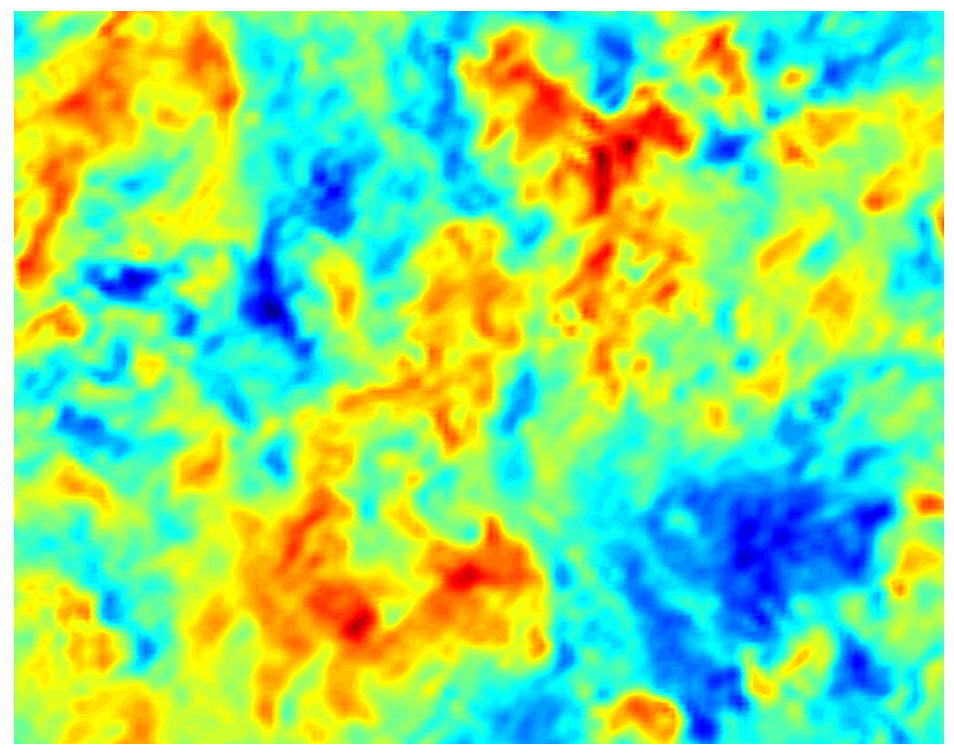
\includegraphics[width=\textwidth]{DNS_Velocity_Field.png}

		DNS Velocity Field
	\end{center}
\end{figure}
\end{column}
\begin{column}{0.3\textwidth}
\begin{figure}[c]
	\begin{center}
		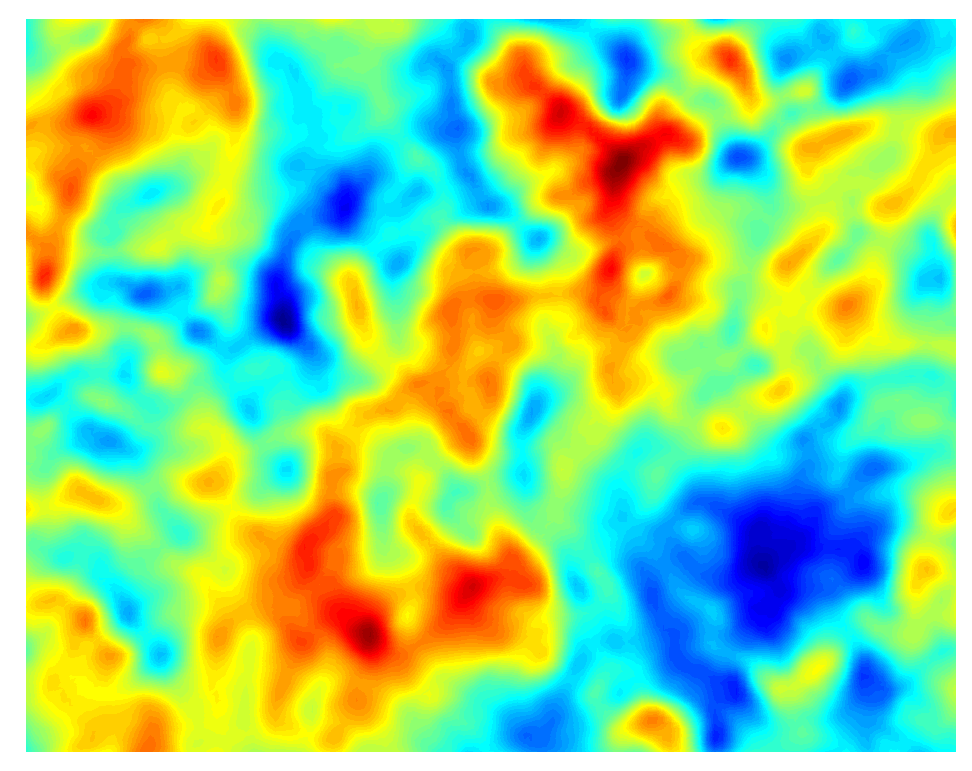
\includegraphics[width=\textwidth]{DNS_Filtered_Velocity_Field_Small.png}

		Filtered Velocity Field $\Delta=L/32$
	\end{center}
\end{figure}
\end{column}
\begin{column}{0.3\textwidth}
\begin{figure}[c]
	\begin{center}
		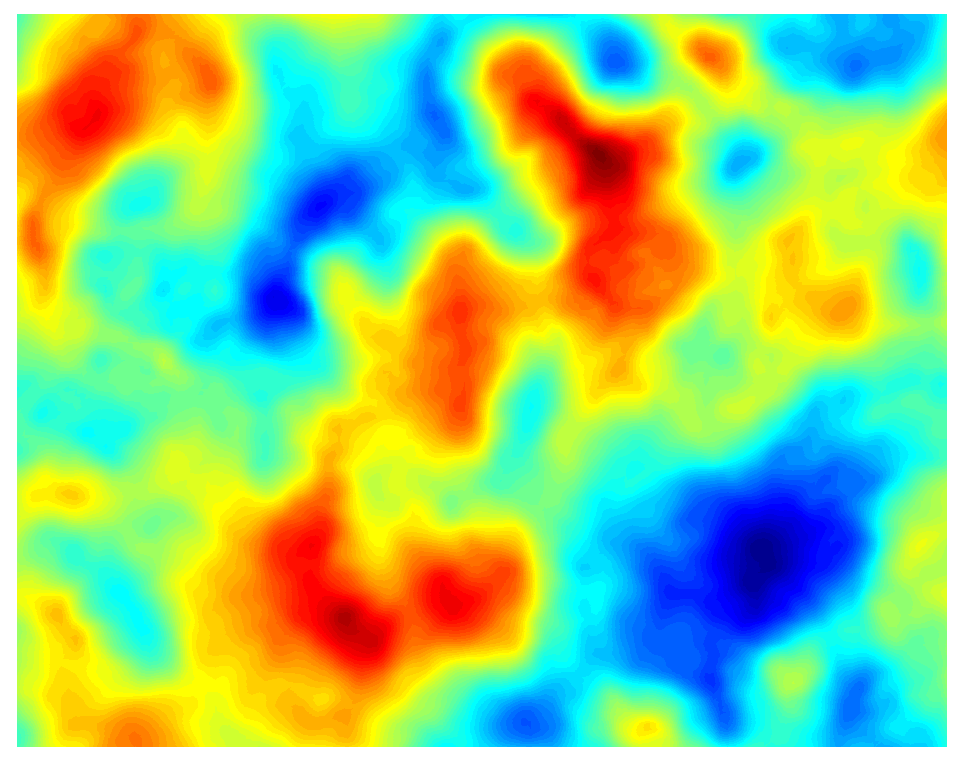
\includegraphics[width=\textwidth]{DNS_Filtered_Velocity_Field_Large.png}

		Filtered Velocity Field $\Delta=L/16$
	\end{center}
\end{figure}
\end{column}
\end{columns}
\end{frame}

\end{document}